\documentclass[12pt]{article}

\title{ECE4063 - Image Thresholding}
%\subtitle{Progress Report}
\author{Emmanuel Jacyna - 24227498 \and James Anastasiou - 23438940}
\date{\today}

\usepackage[T1]{fontenc}
\usepackage[utf8]{inputenc}
\usepackage{rotating}
\usepackage{subfig}

\usepackage{graphicx}
\usepackage{tabularx}
\usepackage{float}
\usepackage{amsmath}
\usepackage{listings}
\bibliographystyle{unsrt}


\begin{document}
\pagestyle{myheadings}
  \maketitle
  \tableofcontents
  \section{Introduction}
  This document represents our findings for Assignment 2 of ECE4063. It is organised into three major sections, assumptions, solution documentation, and a discussion of potential improvements to the project.\\
  
  The task at hand is to perform binary thresholding on an image for use in a bionic eye. The target platform is an Altera Cyclone II FPGA. In order to threshold the image, a histogram of the pixel greyscale values is calculated and used to find the 50th percentile grey scale value. This value is then used to decide whether to colour pixels white or black, performing a total threshold.
  
  \section{Assumptions}
  When thresholding images, we assume that an image where 99.9\% of pixels are one value is meaningless to threshold. In the case of the Altera DE2 board with Terasic camera module, the small variation in value is likely to be because of pixel noise. We also believe that as the target is a human vision system, 100\% accuracy is not necessarily the goal, as we prefer an image that makes sense to the human eye. This design decision allowed for a simplification of the logic circuit required to determine the most accurate thresholding value. 
  
  We also assumed that Model Sim testbenches are 100\% completely accurate representations of reality. This assumption was routinely called into question, however after fixing a number of other assumptions, this sole assumption was found to be a valid assumption.
  
  \section{Documentation - Basic Requirements}
  \subsection{RGB to Grayscale conversion}
  There are a number of ways to convert 12bit RGB values into 8Bit Grayscale values, these include taking the average between all 3 colour channels, desaturating the channels or performing a weighted average based on the NTSC standard. Each of these approaches has benefits and weaknesses, our design decision was to approximate the NTSC standard weighted average via fixed shift additions. The decision to approximate the results meant the design did not need to include a multiplier or divider circuit, which significantly improved the potential performance. 3 multipliers were replaced with 6 additions, which if optimised appropriately could utilise Carry Save Adder hardware to improve the performance. Unfortunately as a result of approximating the NTSC values, the actual grayscale values produced to not match exactly with the theoretical values, this was found to be incorrect by a maximum of 6 units, which we determined to be not a significant loss in precision compared to the speedup and simplification of hardware seen.

  \subsection{Total Histogram}
  The Total Histogram is the overall module responsible for managing the histogram generation, cumulative histogram generation, histogram storage and retrieval. This module is implemented as two-tiered state machine, providing states and certain substates to handle particular edge cases that arose during testing. This module responds to changes of frame valid and data valid signals to determine whether to calculate the histogram or total histogram, or provide direct read through capabilities.

  \subsubsection{Histogram Module}
  The histogram module provides a wrapper around a single port ram with read while write capabilities. The module is implemented via simple pipelining to minimise the latency of the circuit. The module uses a 20bit wide RAM with 256 addresses in order to calculate the Histogram. The actual operation of the module is rather simple, with only a single edge case to handle, which is introduced by the registering of the output from the ram. This potentially introduces a race condition where an old value is read from the ram before the new value has been written, this is overcome by checking for this condition, and incrementing the registered value by 1 before writing again, as well as holding the registered value and checking if the same situation occurs again. By solving this race condition the histogram always produces the correct number of values.

  Additionally the histogram module also handles clearing it's internal ram, which simplifies the interface for connection to the cumulative histogram module.
  
  \subsubsection{Module Testbench Results}
  
  \subsubsection{Cumulative Histogram Module}
  The cumulative histogram is significantly more complex than the histogram module, as it is responsible for a number of \textit{administrative} or \textit{house keeping} tasks. The cumulative histogram iterates over the entire contents of the Histogram ram, cumulating the output and storing the result into another RAM for reading by the histogram display modules. Whilst the cumulative histogram module writes the cumulative values, it also stores the normal histogram values into one of two RAM's. This enables the stored RAM to be used for diaply on the next frame whilst the new histogram is being calculated.

  \subsection{Thresholding Module}
  \subsubsection{Description}
  The thresholding module is very simple. All it needs to do is take in an 8 bit greyscale value and output either a white (255) if the value is above the threshold, or a black (0) if the value is below the threshold. This is accomplished by hooking up a comparator to a multiplexer.
  
  \subsubsection{RTL Diagram}
  \begin{figure}[H]
    \centering{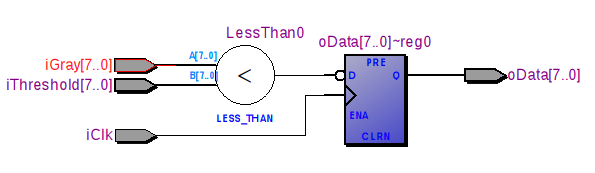
\includegraphics[scale=.8]{Images/ThresholderRTL.png}}
    \caption{Thresholding module RTL}
    \label{fig:thresholder_rtl}
  \end{figure}
  
  
  \subsection{Displaying things}
  \subsubsection{Description}
  In order to display the greyscale image, histogram, cumulative histogram, and thresholded image, we wrote a module to handle multiplexing between them using the switches on the DE2 board, called Arbitrator. This module takes in pixel outputs from the various modules and multiplexes them depending on the switch positions. In order to display images, we simply piggyback on the \(X\_Cont\) and \(Y\_Cont\) signals and modify the \(wr1\_data\) and \(wr2\_data\) inputs to the SDRAM with the appropriate pixel data. \\
      
  Displaying the actual histogram data requires slightly more effort. First we need to extract the histogram data from the histogram RAM and convert the histogram bin contents into pixels for display on the screen. To do this we have a module called HistogramDisplayer. This module takes in the \(Y\_Cont\) signal and uses it to index the histogram RAM. Based on the value obtained from the RAM, it scales the histogram value, and uses the \(X\_Cont\) signal to determine the length of the line to be displayed. 
  \subsubsection{RTL Diagram}
    \begin{figure}[H]
    \centering{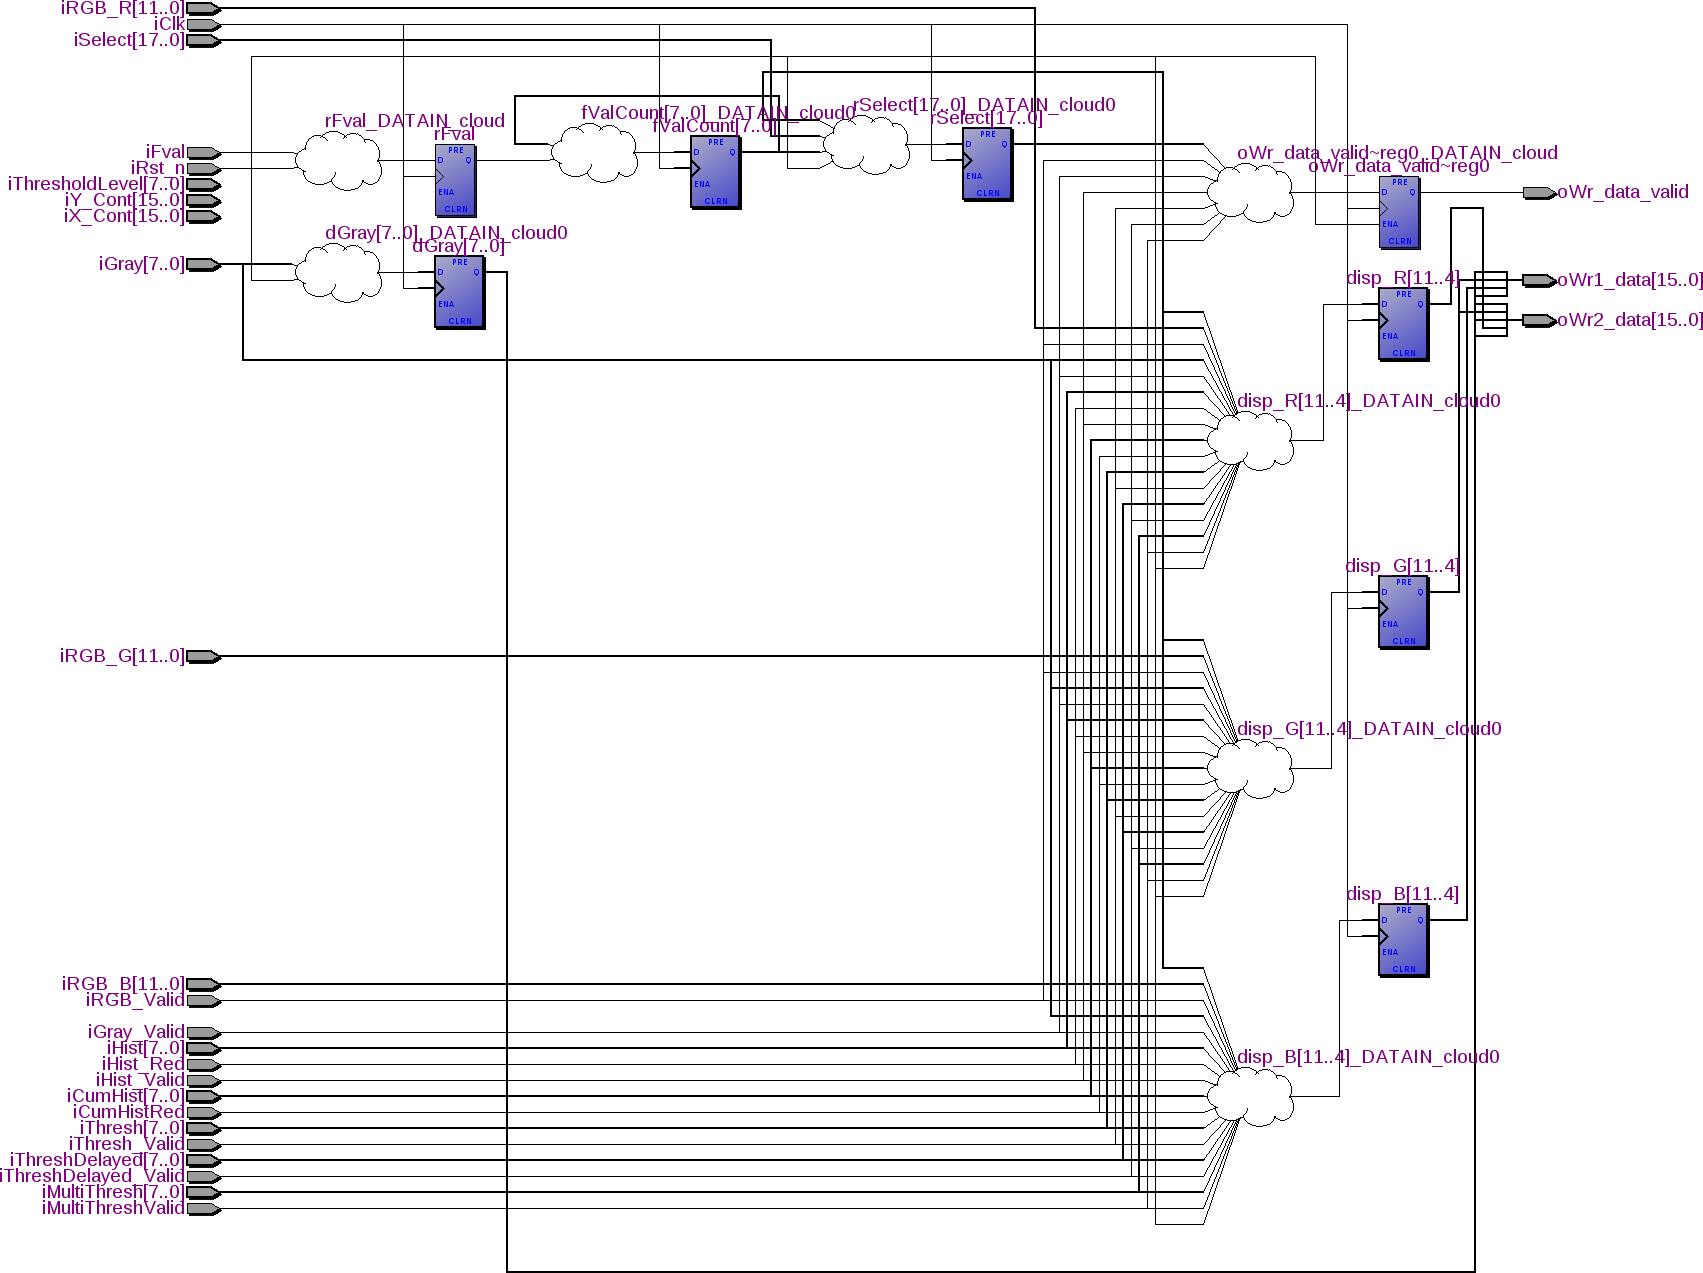
\includegraphics[scale=.8]{Images/ArbitratorRTL.png}}
    \caption{Arbitrator module RTL}
    \label{fig:arbitrator_rtl}
  \end{figure} 
  \subsubsection{RTL Diagram}
    \begin{figure}[H]
    \centering{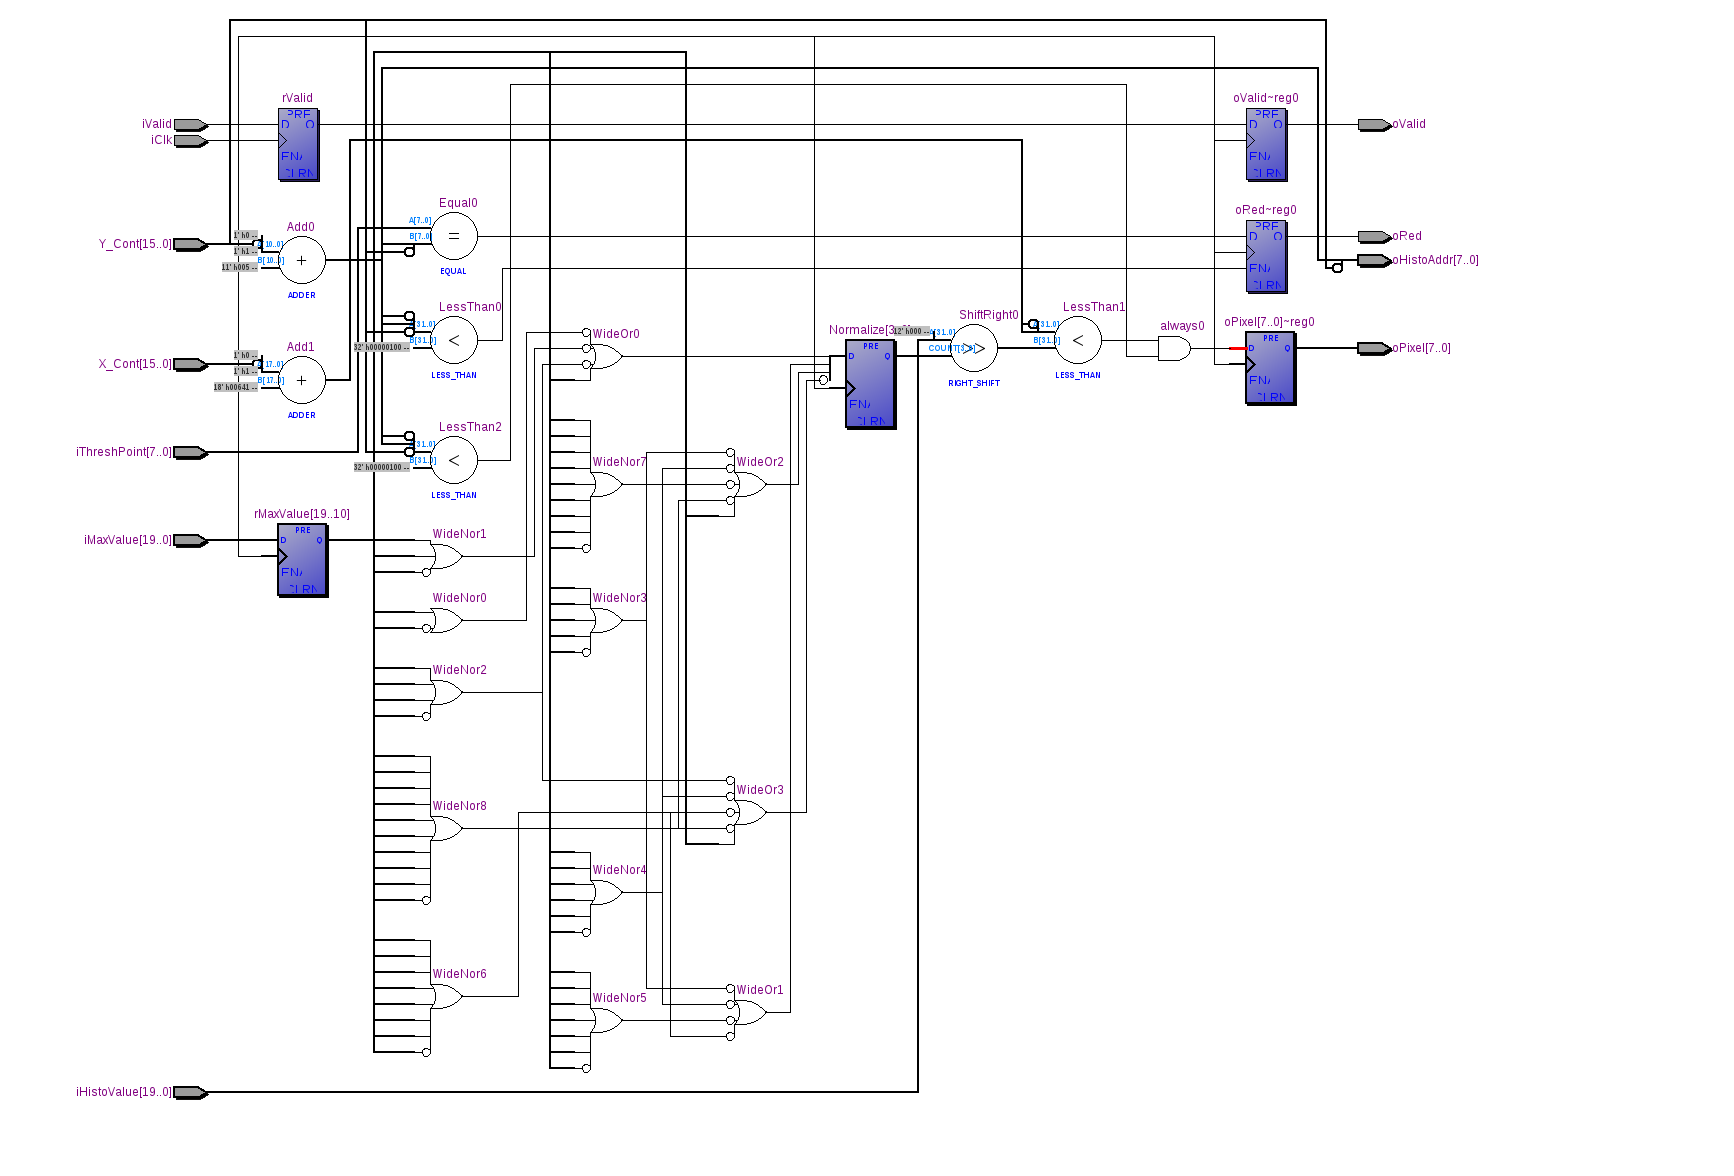
\includegraphics[scale=.8]{Images/HistogramDisplayerRTL.png}}
    \caption{HistogramDisplayer module RTL}
    \label{fig:histogram_displayer_rtl}
  \end{figure}
  
  \section{Documentation - Advanced Requirements}
  A summary of how the advanced requirements were achieved
  
  \subsection{Threshold and Display the Correct Frame}
  In order to successfully threshold the frame the theshold was calculated for, we notices that the \(wr1\_data\) and \(wr2\_data\) wires were not fully packed, and that there was exactly 8 bits of available space that was not utilised. We then recognised that in order to threshold the correct frame, the only information that needs to be delayed that can't be stored on chip was the grayscale values of the image. With this in mind we delayed the gray value and packed the \(wr1\_data\) and \(wr2\_data\) wires with the relevant grayscale values.

  On the read side of the SDRAM FIFO, we intercepted the data, unpacked it and ran the resulting grayscale through a thresholder which utilises a stored threshold value generated by the total module. We only enable display the threshold interception when the appropriate switch is high, thus providing the delayed outcome.

  \subsection{Divided Threshold}
  In order to divide the display into 2 equal subwindows of half width.


  \section{Acknowledgements}
  
  \section{Improvements}
  
  \section{Conclusion}
  
  \newpage
  \section{Appendix A}
  \subsection{RTL Diagrams}
  \subsubsection{Histogram}
  \begin{figure}[H]
    \ContinuedFloat
    \centering{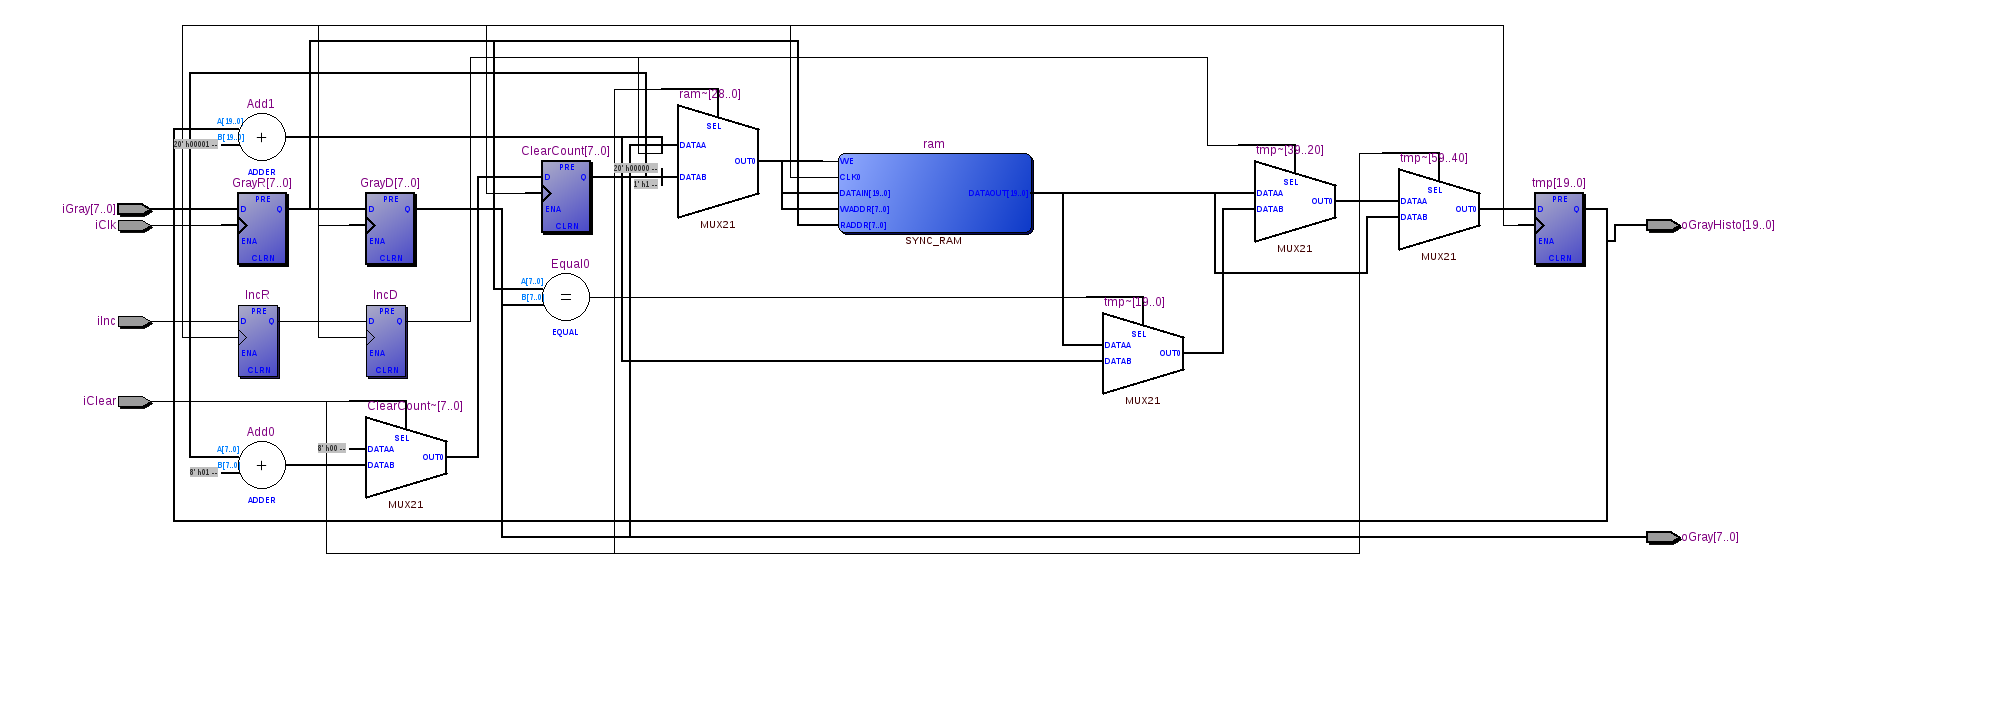
\includegraphics[scale=.6, angle=-90]{Images/HistogramRTL.png}}
    \caption{Histogram module RTL}
    \label{fig:histogram_rtl}
  \end{figure}
  
  
  
  
\end{document}
